\documentclass[publish,JRM,paper]{jaciiiarticle}
\usepackage[dvipdfmx]{graphicx}
% \usepackage[dvips]{graphicx}
\usepackage{epsfig}
\usepackage{color}
% \usepackage{strike}

%%% following commands are unnecessary to edit %%%
\setcounter{page}{1}
\SetVolumeNumber{Vol.29 No.2, 2017}
\SetArticleID{Rb29-2-8252:}
%\SetIndexTab{generalarticle}%specialissue}%   review
%%%%%%%%%%%%%%%%%%%%%%%%%%%%%%%%%%%%%%%%%%%%%%%%%%

\begin{document}

\pagestyle{jaciiistyle}

\title{Excretion Detection System with Gas Sensor\\ \Large{- Proposal and Verification of Algorithm based on Time-series Clustering -}}
\author{Yoshimi Ui*,Yutaka Akiba**,Shohei Sugano**,Ryosuke Imai** and Ken Tomiyama***}
\address{*aba Inc.\\ 3-30-5 Maebara Higashi, Funabashi, Chiba 274-0824, Japan\\ E-mail: yoshimi.wie@aba-lab.com\\
**Chiba Institute of Technology\\ 2-17-1 Tsudanuma, Narashino, Chiba 275-0016, Japan\\
E-mail: \{utahka.akiba, shohei.sugano, rimai.robo.cit\}@gmail.com\\
***Future Robotics Technology Center (fuRo)\\
Chiba Institute of Technology\\
2-17-1 Tsudanuma, Narashino, Chiba 275-0016, Japan\\
E-mail: dr.t@furo.org}
\markboth{Ui, Y. et al.}{Excretion Detection System with Gas Sensor\\- Proposal and Verification of Algorithm based on Time-series Clustering -}
\dates{00/00/00}{00/00/00}
\maketitle

\begin{abstract}% Do not delete this percent symbol
\noindent In this study, we propose an excretion detection system, Lifi, which does not require sensors inside diapers, and we verify its capabilities. It consists of a sheet with strategically placed air intakes, a set of gas sensors, and a processing unit with a newly developed excretion detection algorithm. The gas sensor detects chemicals with odor in the excrement, such as hydrogen sulfide and urea. The time-series data from the gas sensor was used for the detection of not only excretion, but also of the presence/absence of the cared person on the bed. We examined two algorithms, one with a simple threshold and another based on the clustering of sensor data, obtained using the k-means method. The results from both algorithms were satisfactory and similar, once the algorithms were customized for each cared person. However, we adopted the clustering algorithm because it possesses a higher level of flexibility that can be explored and exploited. Lifi was conceived from an overwhelming and serious desire of caretakers to discover the excretion of bed-ridden cared persons, without opening their diapers. We believe that Lifi, along with the clustering algorithm, can help caretakers in this regard.
%please write down your abstract here without first indent
\end{abstract}

\begin{keywords}
Excretion, care, gas sensor, clustering, non-wearing
\end{keywords}

\section{Introduction}
In this study, we propose an excretion-detection sheet, Lifi (hereinafter referred to as Lifi). Lifi was designed to improve excretion care quality without burdening the elderly and handicapped. With this device, caregivers can find and record the presence/absence of in-diaper excretion for diaper changing with appropriate timing. Therefore, the device allows the changing of diapers not in the timing specified by a caregiver, but following the excretion pattern of the cared persons. As cared persons are not left with unchanged diapers, fecal overflow is not a concern. In addition, using this device, it becomes easy to record when the cared persons have excreted; thus, excretion-pattern tables can be created at facilities of any type or scale.

We have developed two major technologies for Lifi. One is a human-body non-wearable technology. If a sensor is placed in a diaper cover, it would directly react against excretion, and excretion detection would be made securely. On the other hand, if a disposable type of sensor is used, it needs to be continuously purchased or washed and placed in a diaper every time after use. Both the continuous purchase and the repeated washing are a burden to nursing homes. Our proposed method entails the use of an excretion-odor \cite{itakura} detection sheet and a gas sensor, and does not require continuous purchase or repeated washing of the sensor. Therefore, the method would be acceptable to nursing homes. For these reasons, our system consists of an air-intake sheet to be put on a bed and a tube connecting to the sheet. Certainly, a new algorithm for odor detection around, and not in, a diaper needs to be developed.

The other is an excretion detection algorithm using a gas sensor. As we aim for our product to be accepted by society, it needs to be a low-cost system. For this purpose, we used a moderately priced gas sensor, which reacted to multiple types of chemicals; however, performances of individual sensors varied considerably. Moreover, as the sensor output largely varied depending on the cared persons, it was found that the algorithm must have a learning capability. Furthermore, this learning capability had to be customized to improve the accuracy of excretion detection. However, it was also found that accurate recording of the presence/absence or the type of excretion with the gas sensor was not feasible at actual nursing care sites; hence, we employed the k-means unsupervised learning algorithm \cite{macqueen,okada,act}, known as the clustering algorithm. As a result, the system was found to be able to detect excretion in several cases, although there was still room for improvement. In the following sections, we will describe this developed system.

\section{Background}
For the improvement of the quality of life (QOL) of the elderly and handicapped, appropriate care for excretion is important. Excretion is a vital function, and caregivers are necessarily involved in excretion care 24 hours a day. As excretion is related to feelings of shame or of compromised dignity in cared persons, caregivers have to pay attention to every single action pertaining to excretion care. Cared persons, such as the elderly or handicapped, may not be able to notify caregivers of in-diaper excretion. Therefore, it could take time until the caregivers notice the excretion, which significantly enhances the onset risk of bedsores (decubitus) or infectious diseases caused by excrement. The discomfort of in-diaper excrement could compel the cared persons to touch the inside of the diaper or to throw the excrement away. This type of behavior is often observed in patients with dementia, and it is called fecal handling.

As explained above, excretion care is highly important. In addition, it casts several psychological, social, or medical problems to caregivers and cared persons. However, no fundamental solution has been offered to these problems, and excretion care is still a burden to both caregivers and cared persons.

To address the above-mentioned problems, caregivers at many facilities regularly change diapers and create excretion-pattern tables. By regularly changing diapers, the caregivers are not required to always inspect the excretion of the cared persons, thus mitigating their burden. On the other hand, the cared persons may not have their diapers changed, even if they had excreted, which could increase the above-mentioned risk of decubitus, infection, or fecal handling. In addition, excrement could exceed the absorption limit of the diapers and could overflow. In cases of fecal overflow or urine overflow, the burden on the caregivers significantly increases. Therefore, one may surmise that regular diaper changing is not always helpful to caregivers. Lifi notifies the caregivers of the timing of excretion to allow diaper changing based on excretion detection.

An excretion-pattern table would be effective; however, its creation requires time, and the burden of keeping a record on the table is significant. Therefore, it can be created only at a limited number of facilities. While an excretion-pattern table needs to be created to reduce the workload of caregivers and improve excretion care, the creation of the table requires labor of the caregivers. Thus, the approach to reduce the burden by using the excretion-pattern table is contradicted. It is desired that all the facilities can create the excretion pattern table at a low cost. Lifi can automatically keep excretion records; it can provide the means to acquire excretion-pattern data without increasing the burden of the caregivers.

\section{Excretion detection}
Various studies have been conducted on devices and systems associated with excretion detection. Excretion detection has thus attracted attention, and the studies and development have progressed toward social implementation; however, they are not sufficient for the widespread use of excretion detection devices.

\subsection{Related studies and products using a gas sensor}
Douguchi et al. \cite{doguchi2}[a] developed a sensor system prototype for detecting the defecation of bed-ridden elderly or handicapped people, and conducted an evaluation test at a clinical site for the purpose of realizing immediate diaper change after defecation. They used three gas sensors, which reacted to three types of gasses, namely hydrogen sulfide, amine compounds, and volatile organic compounds (VOC), and a temperature sensor. A tube and the temperature sensor were attached to a diaper, and the air in the diaper was suctioned through the tube to measure the gas content in the air and the temperature of the air. The data from these four sensors were collectively used to detect defecation. Compared to nonselective gas sensors, which can detect multiple types of chemicals, the selective gas sensors, which can detect only a specific chemical (i.e., hydrogen sulfide or amine compounds), are expensive and cannot be used in commercial products. Moreover, as the temperature sensor and the tube need to be placed inside the diaper, the cared persons may experience discomfort or even feel imperiled owing to the contact of the device with their body.

Mizukawa et al. \cite{mizukawa} proposed an excretion detection system, with the gas sensor TGS2450 of FIGARO Engineering Inc. attached to a diaper. They selected TGS2450 because it was sufficiently compact to reduce user discomfort when attached inside the diaper, and it was inexpensive; therefore, it could be discarded when fouled. Mizukawa et al. performed an experiment on the response time and the heating time property of TGS2450, and found that the detection of urination and defecation was feasible using the gas sensor.
As previously reported, there are studies and products related to excretion detection using a gas sensor. However, these products need to be attached to a diaper, causing discomfort to the cared person. Furthermore, in several cases, the gas sensor is disposed after its use, which raises economic concerns. On the other hand, certain types of products suction and measure the air around excrement to produce measurement data.

Four Leaves Inc. developed a system that encompassed a suction pipe to suction urine or excrement and a gas sensor to detect them [b]. A pump with a waterproof filter is used for suctioning; therefore, the sensor is not touching urine or excrement and is not contaminated by them. The system can even detect flatus through a specialized algorithm, which is based on the width of high value period of the gas sensor data. Similar to this system, Lifi suctions air around the excretion for excretion detection. Moreover, Lifi includes an algorithm to accommodate the large variation of the gas-sensor data, which is due to the individual dispersion of the sensor or users.

\subsection{Products related to excretion detection}
Various systems have been proposed as products or patents related to excretion detection \cite{tamura,ziai}[c-i]. In particular, Tsuruhara[g] proposed a system for detecting urine amount and in-diaper excretion, and developed a detection algorithm to solve the problems of previously proposed method of calculating the amount of urine by integrating temperature changes obtained from a temperature sensor. This method presented difficulty in processing urination data for the second time in a similar manner to the first time because of the specifications of the system. To address this problem, Tsuruhara proposed the attachment of multiple temperature sensors to a diaper and the use of an algorithm of weighted addition of the peak values from the sensors.

Sakurai, Someya, et al. developed a soft, wireless organic sensor to set inside a diaper \cite{fuketa}. They used this sensor for a water-detection sensor sheet, which could be placed in a diaper. Data can be wirelessly collected from the sensor sheet; thus, without a cable, users can move freely.
In addition, there are other products for excretion detection. Certain researchers performed excretion detection by attaching sensors, including a temperature sensor, inside and outside a diaper.
\section{The Lifi excretion detection sheet}
Lifi is a system that can detect the condition inside a diaper, without the need to open it.

\subsection{The Lifi excretion detection sheet}
The Lifi system overview is shown in {\bf Fig.\ref{system}}. The entire system is shown in {\bf Fig.\ref{system}(a)}. The odor is suctioned from the sheet unit, {\bf Fig.\ref{system}(b)}, and is then sent to the sensor unit, {\bf Fig.\ref{system}(c)}. In addition, there is a processing unit for the processing of the obtained data. Thus, the system consists of the three units. TGS2602 [j] of FIGARO Engineering Inc. was employed as the gas sensor; TGS2602 is a gas sensor developed for air quality control and can react to multiple types of chemicals, such as VOC, ammonium, and hydrogen sulfide. Therefore, it is non-selective to specific chemical substances. The steps of the excretion detection process of Lifi are the following.

\begin{figure}[t]
  \centering
  \includegraphics[width=9cm]{./fig/system_fig.eps}
  \caption{System overview of Lifi\newline a.Schematic,b.Sheet unit on bed,c.Sensor unit}
  \label{system}
\end{figure}
\begin{enumerate}
  \item A tube is connected to a suction hole on the sheet. A micro-blower of the sensor unit suctions air through the tube.
  \item As the blower suctions the air through the tube from the sheet, the air is sent to the sensor unit.
  \item Gas sensor TGS2602 mounted in front of the blower senses the delivered air and transmits measurement data to the processing unit.
  \item The processing unit uses an algorithm, which will be described below, to analyze the excretion data, detect the excretion, estimate the excretion type, and send a result.
\end{enumerate}
Thus, the non-wearable system performs excretion detection by acquiring the air from the suction hole on the sheet and measuring the air odor.
\subsection{Method of use}
\begin{figure}[t]
  \centering
  \includegraphics[width=8cm]{./fig/howtouse.eps}
  \caption{Use of Lifi}
  \label{howtouse}
\end{figure}
{\bf Figure \ref{howtouse}} illustrates the method of use of Lifi.

\begin{enumerate}
    \item Lifi is placed on a bed that is used by a cared person, and the cared person lies on it.
    \item When the cared person excretes, Lifi sends a signal to a dedicated tablet in the care station and to dedicated mobile terminals of caregivers to notify them of the excretion.
    \item The terminal receives the notification signal from Lifi and informs a caregiver of the arrival of the signal.
    \item Then, the notified caregiver proceeds to change the diaper.
\end{enumerate}

\subsection{Non-wearable}
As mentioned above, Lifi has a suction hole on its sheet-type hardware for excretion detection, and suctions the air from the hole to measure the air odor by using the gas sensor. Doguchi et al. also used a gas sensor in their excretion detection system \cite{doguchi2}[a]. However, their system requires that a tube be directly inserted into a diaper to measure the odor inside it. Furthermore, a temperature sensor needs to be installed in the diaper. Their system is, therefore, of a wearable type.

Several of the previous types of excretion-detection devices directly or indirectly contact the body of the user \cite{mizukawa}[c]. The excretion-detection devices that tightly come into contact with the body of a cared person could cause discomfort or decubitus because of contact with a foreign object. As Lifi, the non-wearable device, suctions excretion odor from the suction hole on the sheet-type hardware to the gas sensor, the cared persons can use it without concerns about decubitus, sensing a foreign object, or discomfort.

\subsection{The Lifi excretion detection sheet}
As Lifi is developed for actual application at clinical sites, the same algorithm needs to be used for several cared persons. However, TGS2602 presents a relatively large individual dispersion, as shown in {\bf Fig.\ref{tgs2602}}. In the figure, the vertical axis represents the sensor output voltage and the horizontal axis represents the time of the day. The figure shows the sensor output of five examinees during a certain day. The sensor unit was set to yield, every 10 seconds, the average value of the last 10 seconds. This specification was determined after various trials and errors. The odor of excretion varies from person to person; therefore, simple odor detection using a threshold is difficult. Hence, we studied the use of supervised learning to classify the excretion data.

\begin{figure}[t]
  \centering
  \includegraphics[width=8cm]{./fig/graphfig3_1.eps}
  \caption{Excretion data obtained with TGS2602 during one day, for five examinees.}
  \label{tgs2602}
\end{figure}
At the initial stage of the study, for which data collected from healthy examinees at a laboratory were used \cite{matsumoto}, relatively stable signal data were obtained from the gas sensor, and the local features of the signal could be used. Moreover, we had recorded the event (urine, excretion or flatus) and its corresponding gas data; hence, we could use supervised learning. However, data collected at a nursing home presented large variation in sensor signals. Thus, we decided not to use the local features of the signals, but to use global features. It was also found practically impossible to record a correct match between the events and their corresponding gas sensor responses at actual clinical sites. Therefore, instead of acquiring supervised data, Lifi detects excretion and identifies its type from the partial time-series data of the excretion data using the unsupervised k-means method.

\section{The Lifi excretion detection sheet}
{\bf Figure \ref{algo_flow}} shows an outline flowchart of the excretion detection algorithm. The algorithm employed by Lifi consists of a pre-processing unit, an in-bed judgment unit, and an excretion detection unit. In the present study, we examined and evaluated two types of excretion detection units. They are referred to as excretion detection units I and I\hspace{-.1em}I. The excretion detection algorithms containing excretion units I and I\hspace{-.1em}I are called excretion detection algorithm I and I\hspace{-.1em}I, respectively. The two algorithms use the same pre-processing unit and in-bed judgment unit, but different excretion detection units.

\begin{figure}[t]
\centering
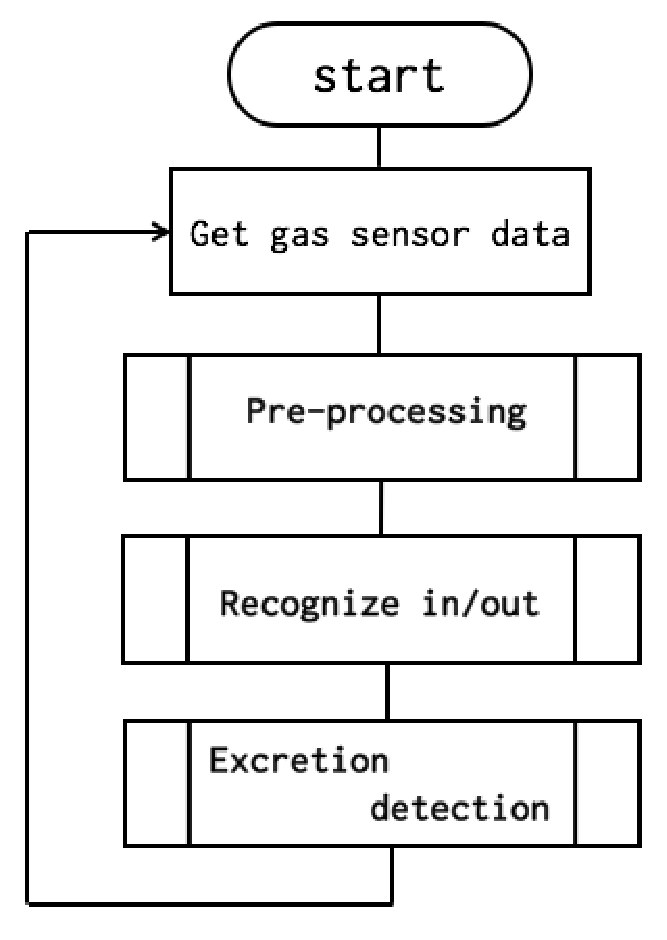
\includegraphics[width=5cm]{./fig/algoflow.eps}
\caption{Overall flow chart of the excretion detection algorithm.}
\label{algo_flow}
\end{figure}

\subsection{Preprocessing unit}
The preprocessing unit renders the excretion data smooth via a moving average. As the response of the gas sensor to the excretion requires approximately 1 or 2 hours to become stable again after the first rise, data clustering can be performed using not an instantaneous feature pattern, but a relatively long-time feature pattern. According to our study and empirical laws, the moving average for over 50 seconds was found to be optimal. However, we used an average of over 1 minute in the experiments because it was more convenient, and the extension of the average period had little influence on the results.

The algorithm divides the moving-average data to partial time-series data of 15 minute, which are then used as a window for in-bed judgment and excretion detection. In the present study, this window is called the sliding window.

\subsection{In-bed judgment unit}
The in-bed judgment unit determines whether a user lies on the Lifi sheet or not. In some cases in the verification experiments, the system issued notification of odor that did not originate from excretion, even when the examinee was not in bed. The purpose of the in-bed judgment was to prevent the system from issuing this type of notification and submitting false reports.

Use of a highly accurate in-bed judgment sensor would render the excretion detection more accurate. However, as our developed detection unit is destined for commercial use, it is necessary to minimize the cost. From this perspective, if the in-bed judgment can be made not with a dedicated in-bed judgment sensor, but with the sensor already used for excretion detection, the product advantage of the system would increase. Therefore, we used the gas sensor for the in-bed judgment.

\begin{figure}[t]
\centering
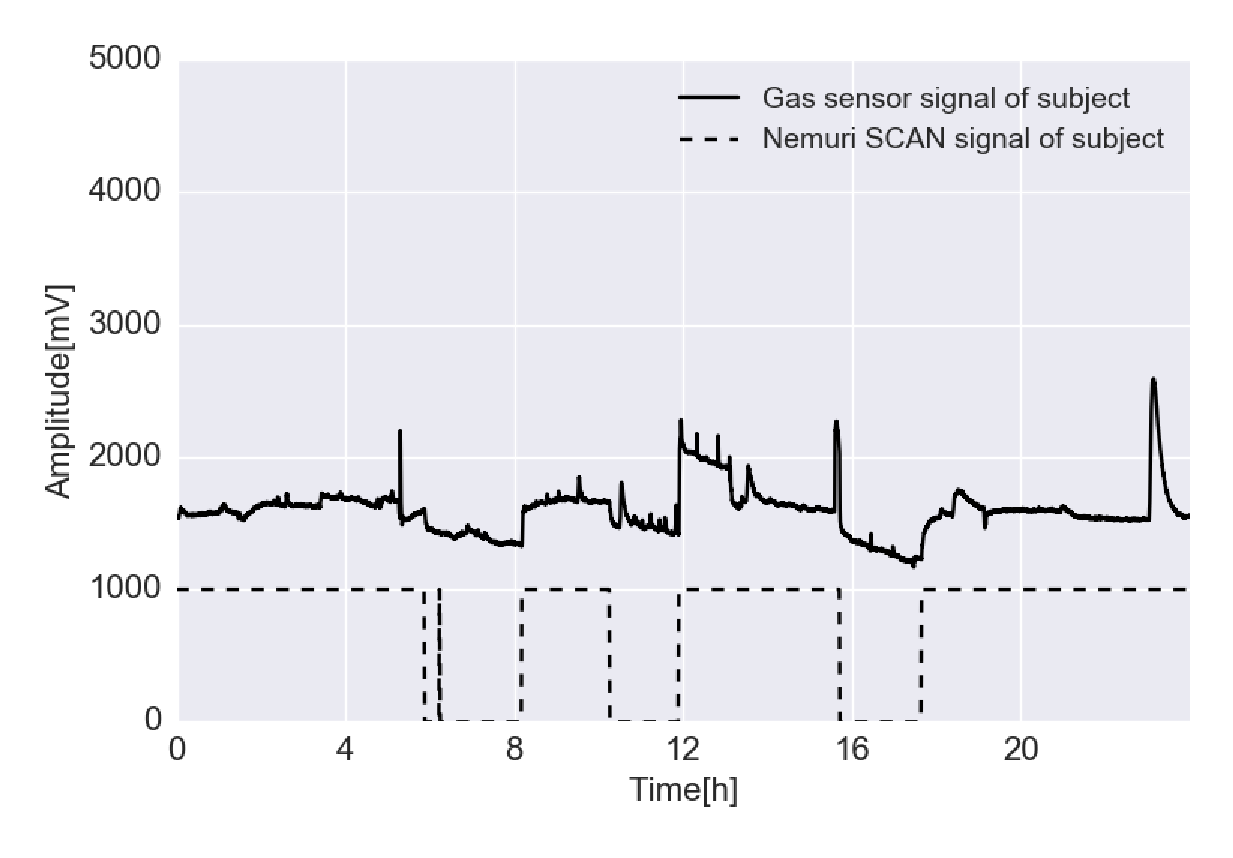
\includegraphics[width=8cm]{./fig/inout3.eps}
\caption{Comparison between excretion and Nemuri SCAN data.}
\label{inout1}
\end{figure}
{\bf Figure \ref{inout1}} shows the moving-average excretion data and the data acquired with the Nemuri SCAN [k] of Paramount Bed Co., Ltd. based on the time stamps contained in both data. The Nemuri SCAN—a device inserted under a mattress—can monitor sleep conditions. It can provide in-bed judgment data and be used to evaluate the in-bed judgment unit. As can be seen in {\bf Fig.\ref{inout1}}, the baseline of the gas sensor data, which is defined as the smoothed gas sensor value after the spikes have been removed, changes when the examinee is in or out of the bed. Therefore, if the baseline of the excretion data can be extracted, one can make in-bed judgment using the gas sensor.

However, excretion data from gas sensor TGS2602 present variation in the baseline values while users are in or out of bed, owing to the individual dispersion of the sensor or to the difference in the body odor of users. Even if the baseline can be correctly extracted, it is difficult to distinguish the in-bed condition from the out-of-bed condition only by using the baseline data because of the variation in the excretion data. We therefore focused on the life pattern of the cared persons, and statistically extracted the mode in each period to make a judgment on the in-bed condition.

In this work, the gas sensor value that is most frequently obtained at each 1 minute interval is called mode. For example, let us assume that a cared person lies in bed at 14:30 almost every day and a relatively high gas-sensor value of approximately 1,200 millivolts, compared to the case where he/she is out of the bed, is frequently observed. In this case, the mode at approximately 14:30 should be 1,200 millivolts. Therefore, we created a histogram for each time; 86,400 seconds of a single day are divided into frames of a certain width, and a histogram is created in each frame. The frame width and the bin width of the histogram need to be set as parameters; in the present study, they were set to 900 seconds and 50 millivolts, respectively. The histograms in the frames are aligned in a single figure, similarly to a spectrogram, where the horizontal axis is the time, the vertical axis is the gas sensor value, and the histogram values are presented with different shades. We call this figure a mode extraction matrix.

An example of a mode extraction matrix created from the two-week excretion data is shown in {\bf Fig.\ref{hist-spectrogram}}. As the mode is different from time to time, one can consider that the mode extraction matrix presents the life pattern of the cared persons. Furthermore, because the mode extraction matrix can accommodate abnormal values, the mode presents a baseline. Therefore, if we use k-means for the clustering of a series of the modes, we should be able to find an in-bed and out-of-bed cluster of the gas sensor values, which can be used to make the in-bed judgment.

The clusters with a large center of gravity should be assigned as the clusters for the in-bed condition, and those with a small center of gravity as the clusters for the out-of-bed condition. Here, the center of gravity is an average vector of each cluster. The following steps show the procedure of distinguishing the in-bed condition from the out-of-bed condition by using the mode.

\begin{figure}[t]
\centering
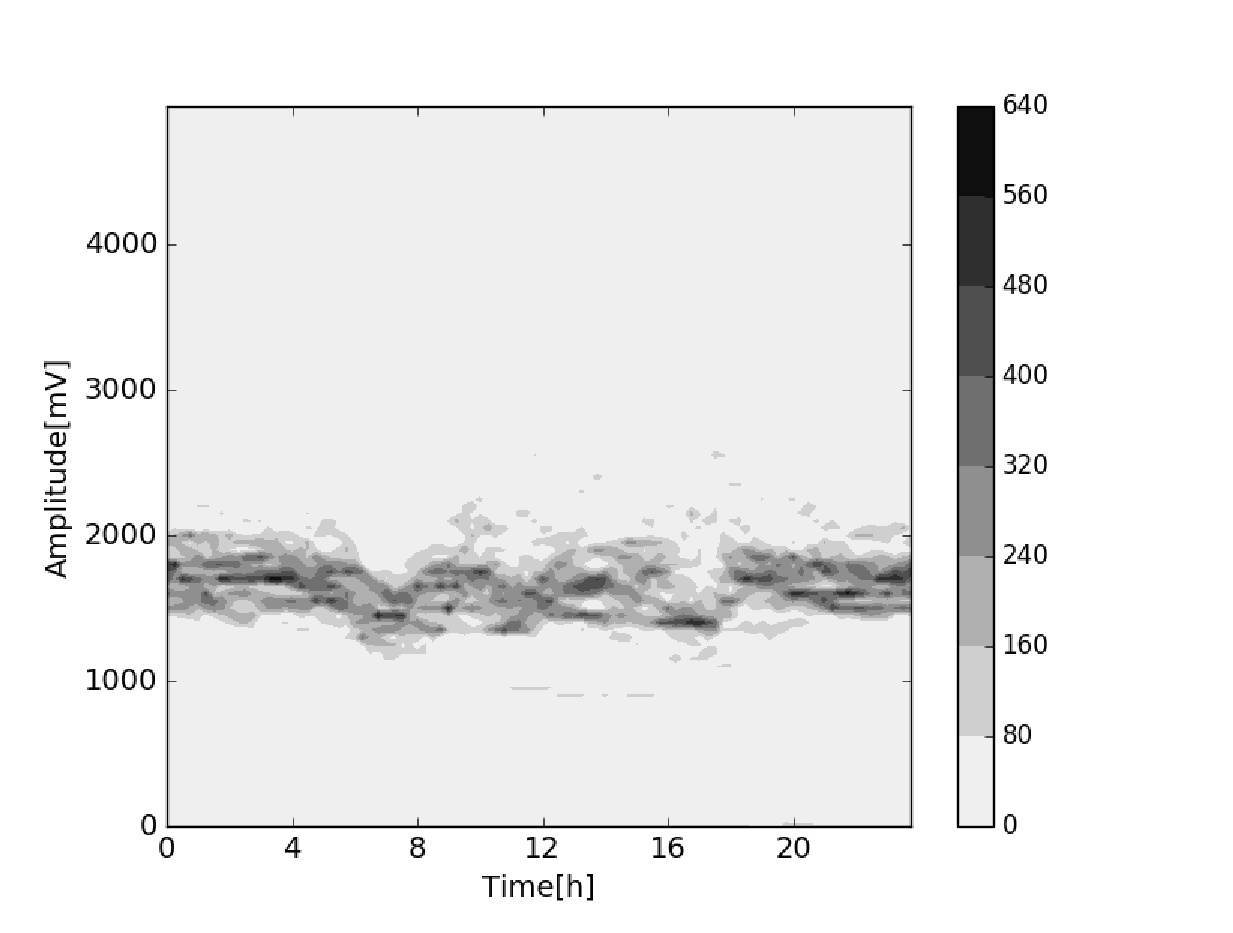
\includegraphics[width=10cm]{./fig/C_matrix.eps}
\caption{Example of mode extraction matrix created by placing histograms along the time axis.}
\label{hist-spectrogram}
\end{figure}

\begin{enumerate}
\item Excretion data, which have been divided in partial time series by sliding windows, are provided.
\item The values in a window are evaluated to determine to which of the two clusters—classified in advance by k-means—the values belong.
\item The examinee is considered to be in bed if one third or less of the values in a window belong to the “out-of-bed” cluster; otherwise, the examinee is considered to be out of bed.
\end{enumerate}

\subsection{Excretion detection algorithm I}
A simple flowchart of the excretion unit in excretion detection algorithm I (hereinafter referred to as algorithm I) is shown in {\bf Fig.\ref{cluster1}}. Algorithm I detects excretion by successively evaluating the excretion data, divided by the sliding windows into partial time-series values. A threshold, which has been determined based on the clustering of the in-bed judgment unit, is used for the evaluation.

The in-bed judgment unit performs data clustering for in-bed clusters and out-of-bed clusters. In addition, the clusters were usable for the detection of abnormal values. If a data area whose data values were higher than the center of gravity of the in-bed cluster by 200 millivolts or occupied one third or more of the window length, the sliding window was regarded as an abnormality-detected window. These threshold values were determined empirically, as shown below. After several trials, we found that the difference of the sensor output between the two clusters was approximately 400 millivolts. Hence, the threshold value of 200 millivolts, which corresponded to half of the difference, was employed. On the other hand, we focused on the point in the window at which the value starts increasing and when the value that has already increased in the previous window starts decreasing. Thus, three situations are possible: increase, decrease, and no change in the values. Therefore, we set the other threshold to be one third of the window length. The one-third threshold was also expected to prevent erroneous detection of a sudden abnormal value due to, for example, flatus.

This algorithm performs unsupervised training using past excretion data to determine a threshold and optimize excretion detection for individuals.

\begin{figure}[t]
\centering
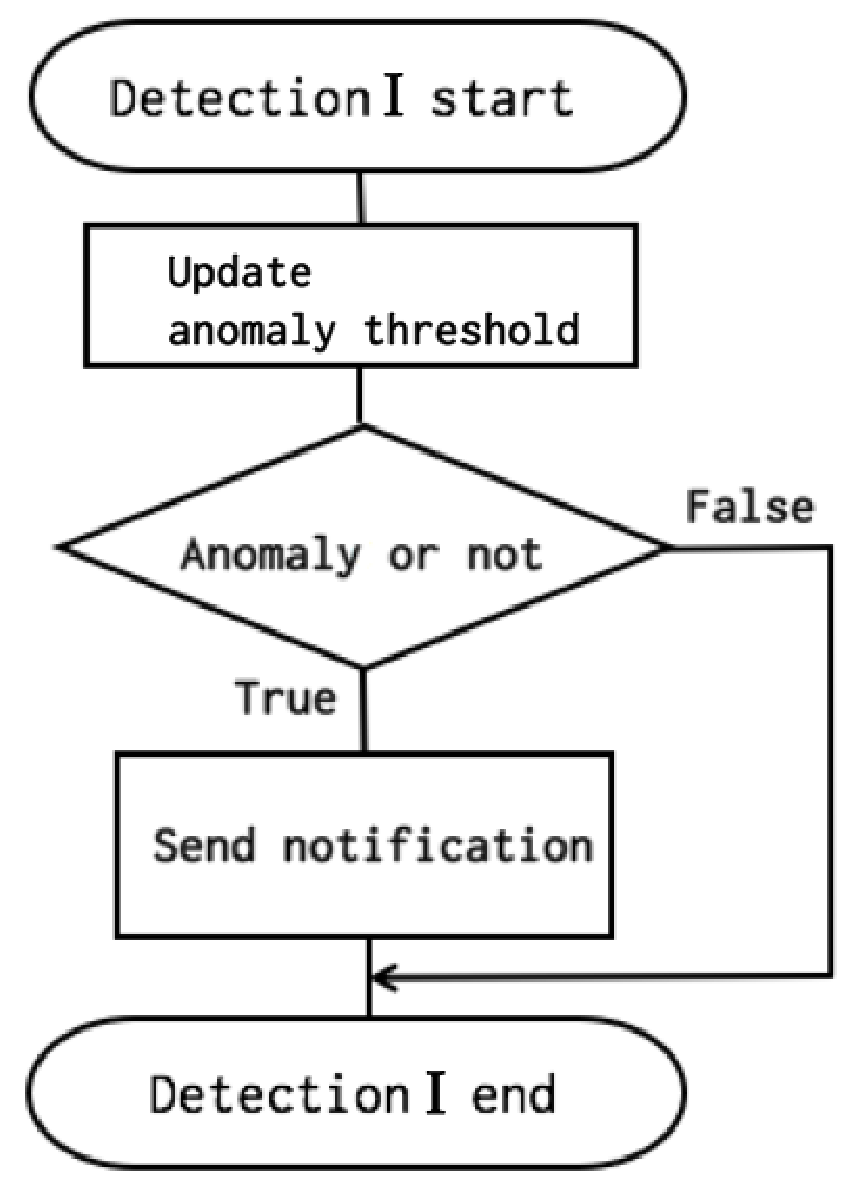
\includegraphics[width=5cm]{./fig/detection1.eps}
\caption{Algorithm I: Clustering by excretion type.}
\label{cluster1}
\end{figure}

\begin{figure}[t]
\centering
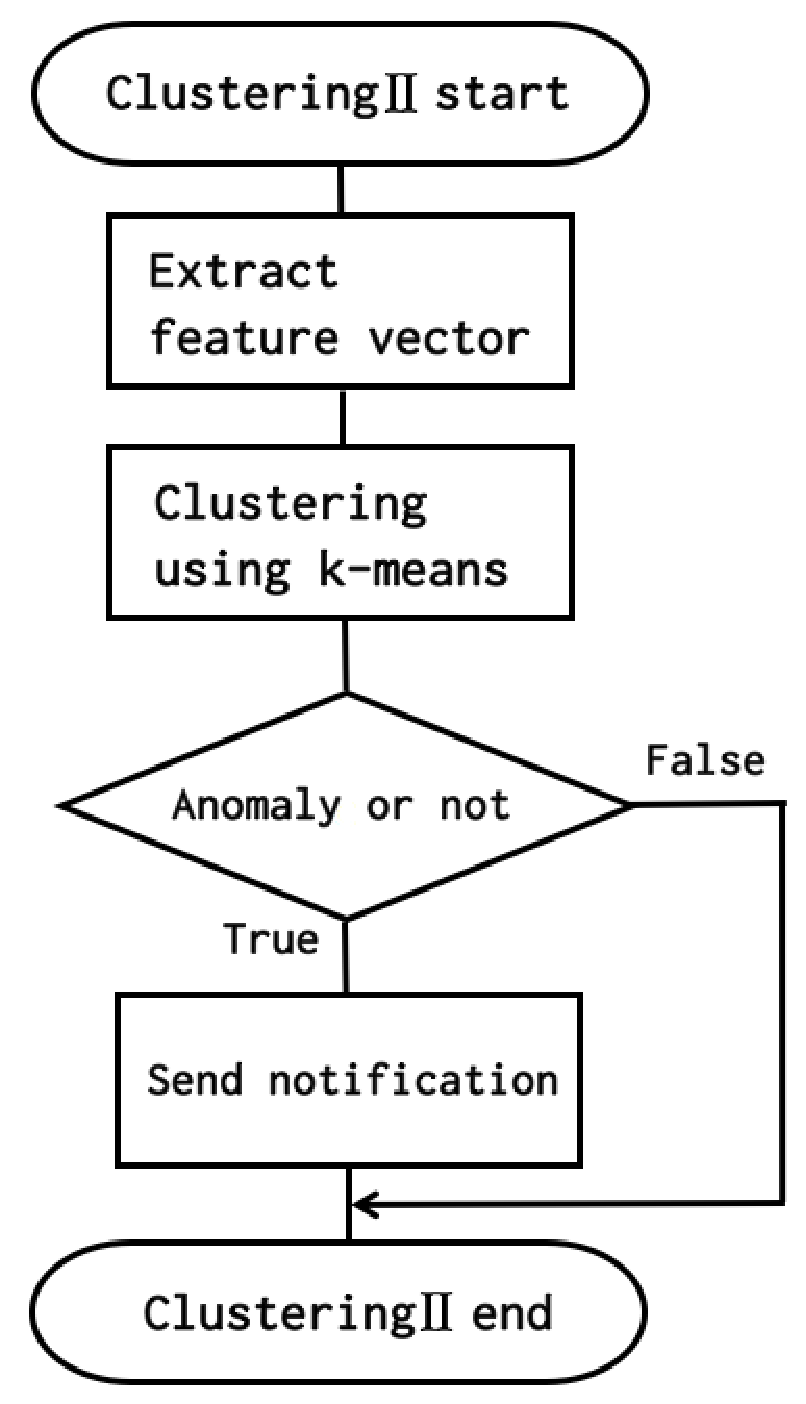
\includegraphics[width=5cm]{./fig/detection2.eps}
\caption{Algorithm I\hspace{-.1em}I: Clustering by excretion type.}
\label{cluster2}
\end{figure}

\subsection{Excretion detection algorithm I\hspace{-.1em}I}
{\bf Figure \ref{cluster2}} shows a simple flowchart of the excretion-type clustering unit with excretion detection algorithm I\hspace{-.1em}I (hereinafter referred to as algorithm I\hspace{-.1em}I). Algorithm I\hspace{-.1em}I extracts features from the sliding window and uses them for the learned k-means model to determine which cluster the sliding window belongs to, whether notification should be made, and what the content of the notification should be. The number of clusters was set to three in the k-means model of algorithm I\hspace{-.1em}I, assuming that there are three types of clusters, namely normal, defecation, and urination.

The feature vector for the k-means model is a five-dimensional vector with the following components: {standard deviation, maximum, minimum, positive area, and negative area}; they are extracted from differential windows in the sliding window. The differential window is a window spanning a target value and one value before. The standard deviation indicates the degree of variation of the data. A large standard deviation indicates abnormality; the maximum and minimum represent the odor level. The positive area is the sum of the positive values in a window, and the negative area is the sum of the negative values in the window. The positive area presents the increasing rate of the original signal waves, as it is the sum of the positive differential value, and the negative area presents the decreasing rate of the original signal waves. The decay of the excretion odor is slower than the urine odor, as the excretion odor source is a solid; hence, the excretion odor could be identified by observing the increasing or decreasing rate of the original signal waves. Hence, we adopted the positive and negative areas as feature vector components.

\section{Excretion data acquisition experiments}
Here, we will describe experiments for collecting sensor data and event records. We used Lifi with algorithm I for the experiments; thus, the experiments also served as performance evaluation for algorithm I. As a result, in certain cases, it was found that the system excessively reacted against flatus, causing a lower detection rate, or did not appropriately handle individual dispersion. On the other hand, it was found that the system was useful for the excretion detection of a person who was found to be in bed by the in-bed judgment.

\subsection{Purpose of experiments}
It is preferable that excretion events be recorded for the entire time span of the gas data collection process. However, this cannot be implemented in practice at actual care facilities. Therefore, we asked a caretaker to open the diaper and check its content when Lifi would send a signal of excretion detection and when the diaper was scheduled to be changed. As mentioned above, we installed algorithm I in Lifi for this purpose; thus, we were able to check algorithm I and to collect data for excretion-detection evaluation. We refer to this series of experiments as an excretion data-acquisition experiment.  The obtained gas data, together with the excretion event records, were stored as CSV files for the ease of further processing.

\subsection{Experimental method}
Lifi was used to collect excretion data from cared elderly persons who predominantly laid in bed, and algorithm I was used to notify caregivers of excretion. The experiment term was five weeks, and the number of the examinees was ten. Although personal data of the examinees are not disclosed here, they were all female within the age range of late 70s to late 80s. Two types of event data, namely excretion events in the regular change of diapers and excretion events when receiving a notification from algorithm I, were simultaneously recorded. However, as caretakers are too busy to keep recording excretion events throughout the day, the data were collected only while the examinees were in bed, from 7 p.m. to 6 a.m. in the next morning. The notification from Lifi was classified into a correct report, a missing report, and a false report, as explained below.

\begin{itemize}
    \item Correct report: Lifi notifies a caregiver of excretion, and he/she actually finds excretion.
    \item Missing report: Lifi does not notify a caregiver of excretion; however, he/she finds excretion.
    \item False report: Lifi notifies a caregiver of excretion, however, he/she did not find excretion.
\end{itemize}
The missing reports are further classified into the following two patterns.
\begin{enumerate}
    \item Hardware error. There is no characteristic feature in the excretion data owing to hardware malfunction, such as failure of suctioning excretion odor because of water-tube clogging caused by dew condensation.
    \item Software error. The excretion data are correctly acquired; however, the excretion event could not be forecasted.

\end{enumerate}
Because an error could occur for other than software-related reasons, the experiment-result evaluation was performed not only for the algorithm, but also for the entire system. Although there could be various influences from hardware errors, we attributed false reports to software errors.

\subsection{Results of the experiment}
In the experiments with the ten examinees, the data from four examinees contained errors due to a hardware damage, as the participated caretakers were not accustomed to handling the experimental apparatus, or due to fecal overflow and sheet contamination. In addition, one of the cared persons fell ill and was hospitalized. Therefore, five examinees could not continue with the experiments, and data from the remaining five examinees were used for the verification of the algorithm.

% table 1
\begin{table*}[t]
\begin{center}
\caption{Excretion detection rate in the excretion data-acquisition experiment, using algorithm I}
\begin{tabular}[t]{c|r|r|r|r|r}
\hline
  Name of examinee & 1st week [\%] & 2nd week [\%] & 3rd week [\%] & 4th week [\%] & 5th week [\%] \\
\cline{2-5}
\hline
A & 16.6 & 0 & 52.3 & 52.9 & 0 \\
\hline
B & 30.0 & 25.2 & 66.7 & 67.7 & 61.5 \\
\hline
C & 52.6 & 60.0 & 44.4 & 42.9 & 47.4 \\
\hline
D & 42.1 & 55.6 & 33.3 & 41.2 & 37.5 \\
\hline
E & 33.3 & 63.6 & 50.0 & 54.5 & 33.3  \\
\hline
\end{tabular}
\label{notification1}
\end{center}
\end{table*}

% table 2
\begin{table*}[t]
\begin{center}
\caption{In-bed and out-of-bed judgment rates in excretion data-acquisition experiments with algorithm I}
\begin{tabular}[t]{c|rrr|rrr}
\hline
  \shortstack{Name of\\examinee} & \multicolumn{3}{c|}{Judgement rates in 4th week [\%]} & \multicolumn{3}{c}{Judgement rates in 5th week [\%]}\\
\cline{2-7}
  & \multicolumn{1}{p{15mm}|}{~~~~~~~~~Total} & \multicolumn{1}{p{15mm}|}{~~~~~~In-bed} & \multicolumn{1}{p{17mm}|}{Out-of-bed} & \multicolumn{1}{p{15mm}|}{~~~~~~~~~Total} & \multicolumn{1}{p{15mm}|}{~~~~~~In-bed} & \multicolumn{1}{p{17mm}}{Out-of-bed} \\
\hline
A & 71.9 & 87.6 & 37.9 & 70.5 & 92.3 & 14.8 \\
\hline
B & 84.1 & 85.0 & 81.8 & 69.8 & 62.0 & 71.6 \\
\hline
C & 83.5 & 94.0 & 56.8 & 86.5 & 98.1 & 56.8 \\
\hline
D & 91.0 & 98.2 & 61.5 & 85.6 & 99.7 & 42.3 \\
\hline
E & 56.1 & 61.0 & 43.7 & 77.7 & 98.3 & 31.3 \\
\hline
\end{tabular}
\label{inout_table}
\end{center}
\end{table*}

In the following sections, we will refer to the examinees as examinees A, B, C, D, and E. {\bf Table \ref{notification1}} lists the excretion detection results of five weeks. The excretion detection rate was calculated from the following formula where NCR and SCFM are the number of correct reports and the sum of the numbers of correct, false and missing reports, respectively.
\begin{eqnarray}
  \mbox{Excretion detection rate}=\frac{\mbox{NCR}}{\mbox{SCFN}} \label{haisetsu}
\end{eqnarray}
{\bf Table \ref{inout_table}} lists the evaluation results of the in-bed judgment of the last two weeks. In these two weeks, the excretion data could be sufficiently collected to be used in the k-means algorithm. The total judgment rate, the in-bed judgment rate, and the out-of-bed judgment rate were calculated from the following formulae. The judgements were considered correct, if the judgment result agreed with the Nemuri SCAN data.
\begin{eqnarray}
  \mbox{Total judgement rate}&=&\frac{\mbox{NCC}}{\mbox{TNC}}\\
  \mbox{In-bed judgement rate}&=&\frac{\mbox{NCIB}}{\mbox{NCAI}}\\
  \mbox{Out-of-bed judgment rate}&=&\frac{\mbox{NCOB}}{\mbox{NCAO}}
\end{eqnarray}
Here, NCC, TNC, NCIB, NCAI, NCOB, NCAO are the number of cases for which correct judgements are obtained, the total number of cases, the number of cases for which the in-bed conditions were correctly detected, the number of cases where the examinees were actually in bed, Number of cases for which the out-of-bed conditions were correctly detected, and the number of cases where the examinees were actually out of bed, respectively.
\subsection{Discussion on experiments}
As presented in {\bf Table \ref{notification1}}, the individual dispersion and difference between weeks were extremely large. The data of examinee A contained certain characteristic patterns owing to a hardware error or to limited excretion odor; the excretion rate was zero in some weeks. This indicates the difficulty of system adaptation to the experimental environment or the difficulty faced by the individual examinees in the excretion detection experiments. However, for examinee B, learning of the thresholds could increase the detection rate by more than 60\%. The system functioned relatively well in this case.
The results of the in-bed and out-of-bed judgment rates in {\bf Table \ref{inout_table}} reveal that the in-bed judgment rate was 60\% or higher and, in several cases, over 80\%. Therefore, the mode extraction matrix that focused on the life pattern is effective for the in-bed judgment. However, the in-bed judgment rate significantly varied from person to person. This means that there were many cases where the examinees not lying in bed were detected as being in bed, which could be owing to the influence of the odor around Lifi, when the examinees were out of the bed. On the other hand, when the cared persons were in bed, they lay on the Lifi with comforters, and the measurement values were stable. In this case, the judgment rate was high.
Therefore, it is difficult to further increase the out-of-bed judgment rate by only using the gas sensor, which is easily affected by the odor around the bed when the examinees are out of bed. The rate could be increased by acquiring more information from a humidity sensor, for example. However, we decided that the current rate of the out-of-bed identification is already sufficiently high for the excretion detection unit.

\section{Evaluation experiments for algorithm I\hspace{-.1em}I}
Here, we will describe the evaluation experiments for algorithm I\hspace{-.1em}I. It was found that the dominant cause for the missing reports was a hardware error, and that for the false reports was flatus. The false flatus-related reports increase the workload of the facility staff unnecessarily and should be reduced. Distinguishing flatus from excretion is, therefore, necessary.

\begin{figure}[t]
  \centering
  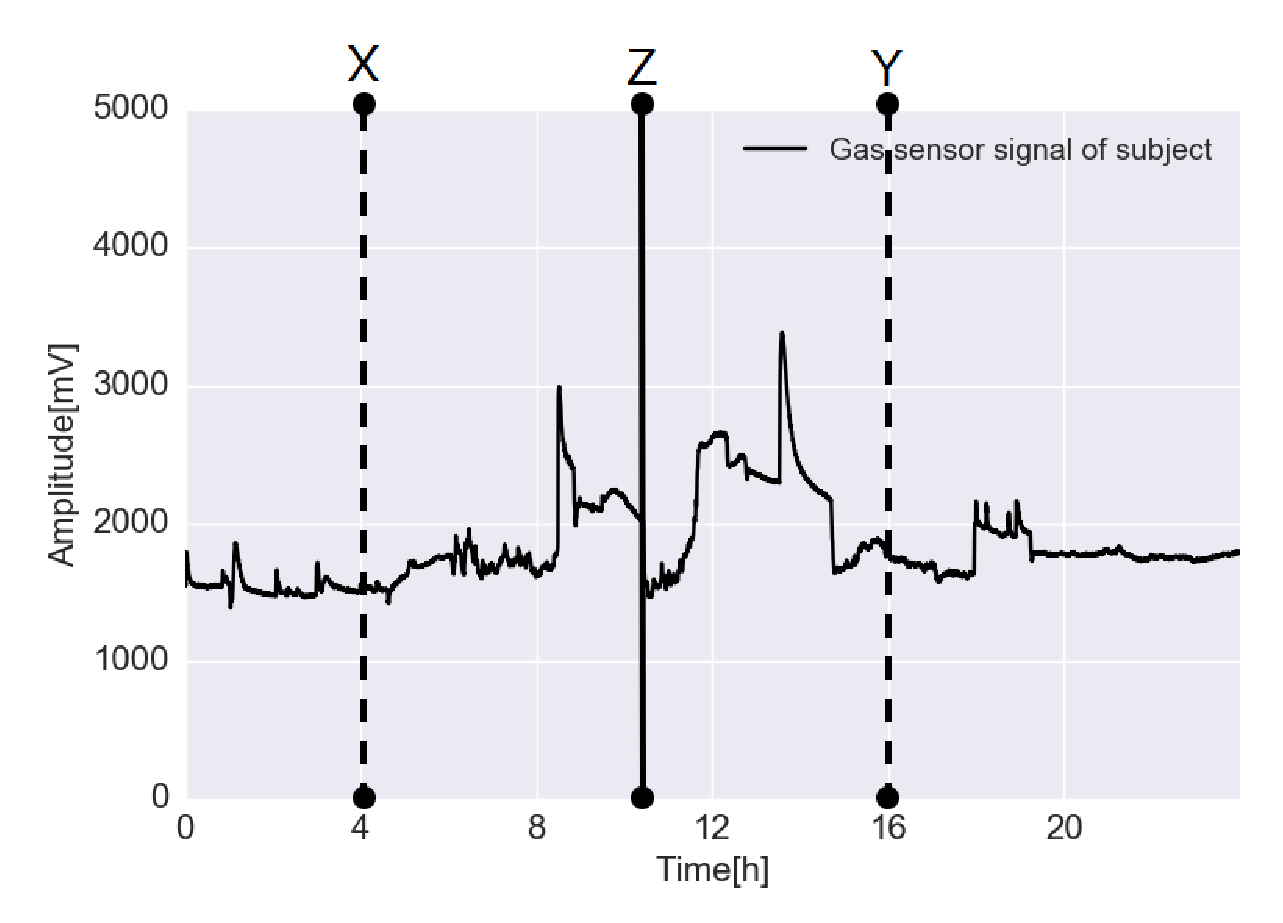
\includegraphics[width=8cm]{./fig/xyz.eps}
  \caption{Example of event X, event Y, and excretion detection Z}
  \label{event}
\end{figure}
\subsection{Experimental method}
As shown in {\bf Fig.\ref{event}}, let us assume that two adjacent diaper-changing events occur (events X and Y) in the excretion data. The excretion report (on the presence/absence of excretion) that is submitted for diaper-change event Y is a correct report, if it agrees with the result of the detection performed during the period between two diaper-change events. A missing report is correct if the report indicates the excretion, but the detection indicates its absence; a false report is correct if the report indicates the absence of excretion, but the detection indicates its presence. The excretion data collected from the five examinees in the last week that were presented in Section 6 were used for the present experiments; the event data that were saved during that time were also used. The learning process of the k-means model uses two-week excretion data collected from the same examinee, from whom one-week excretion data were collected for the excretion detection experiments. By comparing the data with the results of the fifth week of the excretion data-acquisition experiments, the change in the number of correct and missing reports was studied.

\subsection{Experiment result}
The result of the experiment is presented in {\bf Table \ref{notification2}}. The excretion detection rate of the entire system was calculated via (\ref{haisetsu}), considering all the missing reports in the experiments. Therefore, this detection rate is with regard to the Lifi system, not to the software alone; it encompasses both the hardware and software. For the calculation of the excretion detection rate of the algorithm alone, the hardware-caused situations, in which the gas sensor values remained almost the same, were ignored in the entire data to evaluate the performance of the algorithm itself. Then, the remaining data and (\ref{haisetsu}) were used for the calculation of the excretion detection rate of the algorithm. As the data used for the calculation were obtained by intentionally eliminating the data related to hardware problems, only the simple detection rate was calculated.

% table 3
\begin{table}[t]
\begin{center}
\caption{Excretion detection rate in algorithm I\hspace{-.1em}I}
\begin{tabular}[t]{c|r|r}
\hline
  \shortstack{Name of \\examinee} & \shortstack{Excretion detection\\rate of\\entire system [\%]} & \shortstack{Excretion detection\\rate of\\algorithm only [\%]} \\
\hline
A & 30.8 & 100.0 \\
\hline
B & 65.0 & 65.0 \\
\hline
C & 35.7 & 62.5 \\
\hline
D & 20.0 & 62.5 \\
\hline
E & 42.8 & 66.7 \\
\hline
\end{tabular}
\label{notification2}
\end{center}
\end{table}

\subsection{Discussions on the experiment}
The excretion detection rate of the entire system in {\bf Table \ref{notification2}} is almost at the same level as that of the fifth week in {\bf Table \ref{notification1}}, indicating that it was difficult to improve the detection rate by improving the software. Therefore, we examined the data of the time at which the missing report was submitted, and examined whether the missing reports were caused by a software error or a hardware error. The excretion data of the time at which the missing report was submitted were found mostly to have a flat signal with no characteristic pattern, which indicated that the sensor failure of measurement was mostly due to water-tube clogging.

The software can be fine-tuned as well. For example, the result can change depending on the window length or the number of the clusters. In our future studies, it is therefore necessary to select parameter values appropriate to excretion detection.

Moreover, it is necessary to eliminate false reports, which are issued when a characteristic pattern is detected, with no excretion. Most of the false reports could be attributed to flatus. To distinguish flatus from excretion, it is necessary to find a characteristic quantity that distinguishes the excretion signal pattern from the flatus signal pattern, or to change the number of the clusters. These measures would improve the detection accuracy.

\section{Conclusions}
In this study, we reported the research and development of the excretion detection sheet, Lifi. We first described the Lifi system and its method of use. Lifi uses a gas sensor to detect excretion; however, it presents difficulties in accurately recording the details of excretion events. Therefore, unsupervised learning was used to extract and cluster characteristic patterns from the excretion data for excretion detection. The detection accuracy was over 60%, if the influences from the hardware were ignored.

In future, we first plan to reduce the number of false reports and to design a method for distinguishing events such as flatus, which do not require diaper change, from those including excretion events, which require diaper change.

\acknowledgements
The authors would like to sincerely thank the Special Nursing Home for the Aged Sawayaka-en and the Social Welfare Corporation SEISHI for providing them with a location for the experiment. The experiments on excretion, which requires several ethical considerations, could not have been conducted without the significant support of the examinees, their families, and the facility staff. Their daily efforts to liven up the atmosphere of the nursing homes are appreciated. The authors also thank Paramount Bed Co. Ltd., which has been a collaborating company for the development of products, for providing the knowledge and experience on mass production and practical development that the company has accumulated over half a century. Finally, the authors would like to thank the students from the Chiba Institute of Technology for their support in the experiments for the repair and maintenance of the experimental equipment and data collection.

%\bibliographystyle{unsrt}%if you use bibtex
%\bibliography{template}

%[IMPORTANT]
%To clarify research positioning and purpose, authors should survey international literatures,
%including JRM publications, and list them in references. It is strongly recommended that
%authors include JRM publications in references (JRM is under evaluation of SCI to get IF).
%All papers appear in the JRM and PDFs made available free of charge at the following website
%[OPEN ACCESS] at
%https://www.fujipress.jp/jrm/rb/
%Create your account for download for free at
%https://www.fujipress.jp/usces-member/?page=newmember


\begin{thebibliography}{99}
\bibitem{itakura} T. Itakura, M. Mitsuda and T. Tanamura,``Research on Characteristics of the Odors from Excrement at the Adult Diaper Exchange,” J. Environ. Engr. Architectural Institute of Japan, Vol. 73, No. 625, pp. 335-341, 2008. in Japanese
\bibitem{macqueen} J. MacQueen, ``Some methods for classifcation and analysis of multivariate observations,” Proc. Fifth Berkeley Symp. on Math. Statist. and Prob., Vol.1, pp. 281-297, University of California Press., 1967.
\bibitem{okada} S. Okada, K. Hitomi, N. Chandrasiri, Y. Rho and K. Nitta, ``Analysis of driving behavior based on time-series data mining of vehicle sensor data,” Forum on Information Technology FIT2012, 2012. in Japanese
\bibitem{act} T. Ueda, H. Sugimura, K. Matsumoto and M. Isshiki, ``Activity Recognition of the Human from Sensor Data,” The 27th Annual Conference of the Japanese Society for Artifcial Intelligence, 2013. in Japanese
\bibitem{doguchi2} Y. Douguchi, Y. Yonezawa and Y. Yamada, ``Development of the sensor system for defecation,” Heisei 11 Research Report, Industrial Research Institute of Ishikawa, 2000. in Japanese
\bibitem{mizukawa} T. Mizukawa, M. Tahashi, M. Kawashima and H. Goto, ``Development of urination/defecation detector using gas sensor (Poster Presentation),” IEICE Tech. Rep., Vol.115, No.152, WBS2015-13, MICT2015-17, pp. 1-5, July 2015. in Japanese
\bibitem{tamura} T. Tamura, K. Nakajima, et al., ``A warning detector for urinary incontinence for home health care,” Biomed Instrumentation Technology, Vol.29, No.4, pp. 343-349, 1995.
\bibitem{ziai} M. A. Ziai and J. C. Batchelo, ``Smart radio-frequency identifcation tag for diaper moisture detection,” Healthcare Technology Letters, Vol.2, No.1, pp18-21, 2015.
\bibitem{fuketa} H. Fuketa, K. Yoshioka, et al., ``Organic-transistor-based 2kV ESD- tolerant fexible wet sensor sheet for biomedical applications with wireless power and data transmission using 13.56MHz magnetic resonance,” Proceedings, 2014 IEEE International Solid-State Circuits Conference, pp. 490-491, 2014.
\bibitem{matsumoto}N. Matsumoto, ``Noncontact Excretion Detection Sheet Liflm – Construction of The Excretion Detection Algorithm -,” Graduation Thesis, Chiba Institute of Technology, 2014. in Japanese
\end{thebibliography}

\newdimen\bibindent
\setlength\bibindent{1.5em}
\newenvironment{bib}[1]{
  \ssection*{\small Supporting Online Materials:}
  \addcontentsline{toc}{section}{References}
  \vspace*{-10pt}
  \renewcommand\baselinestretch{1}
  \footnotesize
  \setlength{\itemindent}{12pt}
  \setlength{\labelwidth}{3em}
  \setlength{\labelsep}{5pt}
  \list{[\alph{enumii}]}{
    \advance\leftmargin\labelsep
    \itemsep 0pt plus .5pt
    \usecounter{enumii}
  }
  \def\newblock{\hskip .11em plus .33em minus .07em}
  \if@technote
  \sloppy\clubpenalty4000\widowpenalty4000\interlinepenalty100%
  \else
  \sloppy\clubpenalty4000\widowpenalty4000\interlinepenalty500
  \fi
  \sfcode`\.=1000\relax}{\endlist}
\begin{flushleft}
\begin{bib}{99}
\bibitem{a} Industrial Research Institute of Ishikawa, Heisei 11 Research Report http://www.irii.jp/randd/theme/2000/01.htm [Accessed Dec. 7, 2016]
\bibitem{b} Four Leaves Co. Ltd., Urination and defecation detector, Web page http://www.fourleaves.co.jp/product/original02.html [Accessed Sept. 14, 2016]
\bibitem{c} AWAJITEC, NightNox, Web page http://www.awajitec.com/nightnox.html [Accessed Aug. 20, 2016]
\bibitem{d} Teltec Tohoku, Wireless diaper sensor, Web page http://www.teltectohoku.co.jp/houjin/34.html [Accessed Sep 14, 2016]
\bibitem{e} Sensassure, talli, Web page http://www.sensassure.com/\#talli [Accessed Dec. 15, 2016]
\bibitem{f} T. Nakamura, Method of detecting urination and defecation in using paper diaper and the like, Japan Patent, JP2002-233548A, 2002-08-20.
\bibitem{g} M. Tsuruhara and C. Sekine, Device for detecting urine and feces in diaper, WO Patent, WO2011162402A1, 2011-12-29.
\bibitem{h} T. Urabe, Defecation detector, Japan Patent, JP2002143213A, 2001-10-17.
\bibitem{i} Y. Abe, I. Fukuda, et al., Excretion detector, Japan Patent, JP2002159523A, 2002-06- 04.
\bibitem{j} FIGARO, TGS2602, Web Page http://www.fgaro.co.jp/product/entry/tgs2602.html [Accessed Sept. 14, 2016]
\bibitem{k} Paramount Bed, Nemuri SCAN, Web page http://www.paramount.co.jp/contents/951, [Accessed Sep. 14, 2016]
\end{bib}
\end{flushleft}
\appendix

%\newpage
\vspace{25pt}

% *Profiles and photos are not necessarily required at the first submission
% \begin{profile}
%   \Name{Your Name}
%   \Affiliation{Your Institute}
%   \Address{Address of Your Institute}
%   \History{Your History}
%   \Works{$\bullet$ Your Works}
%   \Membership{$\bullet$ Your Learned Societies}
%   %%please place any image files in subdirectory named ``fig''
%   \Photo[\epsfig{file=./fig/photosample.eps,height=93.54pt, width=70.86pt}]
% \end{profile}
%
\end{document}
